
\section{Chassis}


\subsection{Overview}
\subsubsection{Requirements and Constraints}
Paramount among our requirements is the ability of the chassis to withstand the rigors of operation, with a primary focus on supporting a load of up to 250 kg. The chassis must serve as the sturdy foundation upon which all subsystems are mounted. From the propulsion system to the suspension components, every subsystem must find its place within the chassis. A chassis that is inaccessible is as good as useless. Hence, a key requirement driving our design is the ease of access for maintenance and assembly. Components must be readily accessible, allowing for swift troubleshooting and efficient assembly processes. The chassis must seamlessly integrate with the aeroshell, providing a secure mounting point while ensuring aerodynamic efficiency. This requirement necessitates careful consideration of mounting points and structural reinforcements to support the aeroshell without compromising performance. Weight is the enemy of performance, and our chassis must strike a delicate balance between structural robustness and lightweight construction. Utilizing advanced materials and optimization techniques, we aim to minimize weight without compromising strength or durability. While performance is paramount, cost considerations cannot be overlooked. Our chassis must be constructed in a manner that balances performance with affordability, ensuring that our project remains economically viable without sacrificing quality or functionality. The chassis must withstand the dynamic forces exerted by both the braking system and the suspension components. This constraint necessitates careful reinforcement and structural design to ensure that the chassis remains resilient under varying load conditions. The design must incorporate provisions for easy extraction of the battery pack, facilitated by a rail system. This constraint imposes additional design considerations, such as clearance and mounting points, to ensure seamless integration and accessibility.

\subsubsection{Concept}

The chassis plays an important role in any moving structure, providing the structural foundation and support necessary to ensure safety, stability, and functionality for the entire vehicle and all the systems it holds. In this year's iteration, our pod utilises a two-track system, which not only allows for extra room to house subsystems but also lowers the pod's centre of mass, thereby enhancing stability. This design decision results in a wider and consequently shorter pod.

At the core of our design philosophy lies the integration of carbon fiber sandwich plates, a cutting-edge material renowned for its exceptional strength-to-weight ratio and structural integrity.
The foundation of our chassis is built upon a rectangular framework, strategically crafted to optimize both stability and versatility. Covering the entirety of the lower section of the pod is a ground plate, providing a robust foundation while simultaneously enhancing aerodynamic efficiency. This ground plate serves as the backbone of the chassis, ensuring unparalleled stability and structural integrity.
Extending longitudinally from the front to the back of the pod are two key components: the longitudinal plates. These plates constitute the primary structural elements of the chassis, serving as the anchor points for vital components such as the suspension system, brakes, and motor. Crafted with precision and reinforced for maximum resilience, these longitudinal plates epitomize the marriage of form and function, providing the framework upon which our pod's performance hinges.
To further fortify the structural integrity of our chassis and prevent any potential bending or detachment of the longitudinal plates, we have strategically incorporated three additional cross panels. These panels, positioned perpendicular to the longitudinal plates, serve as stabilizing agents, distributing forces evenly throughout the chassis and bolstering overall rigidity. these cross panels ensure that our pod remains steadfast and unwavering, even under the most demanding conditions.
Central to the assembly of our chassis is a plug-in system, integrated into the carbon fiber sandwich plates. Through precision-cut cutouts and advanced adhesive technologies, these plates seamlessly interlock and adhere, forming a cohesive and resilient structure. This plug-in system not only streamlines the assembly process but also enhances the overall integrity of the chassis, ensuring a robust and reliable foundation for our pod.

\subsubsection{Size, Components, and Appearance}
\begin{table}[ht]
\centering

\label{table:components}
\begin{adjustbox}{width=\textwidth,center}
\begin{tabular}{|>{\bfseries}m{2.5cm}|m{1.4cm}|m{1.7cm}|m{2.1cm}|m{2.2cm}|m{2.6cm}|m{2.2cm}|}
\hline
Component & Number & Mass [kg] & Size [mm] & Material & Manufacturing process & In-house/ outsourced \\
\hline
GP & x1 & 1 & 1480x882x20 & CF Sandwich & Waterjetcut & Outsourced \\
CacP & x1 & 1 & 882x200x20 & CF Sandwich & Waterjetcut & Outsourced \\
BacP & x2 & 0.1 & 882x200x20 & CF Sandwich & Waterjetcut & Outsourced \\
BCalP & x2 & 0.2 & 883x200x20 & CF Sandwich & Waterjetcut & Outsourced \\
AalP & x2 & 0.2 & 270x200x20 & CF Sandwich & Waterjetcut & Outsourced \\
Seam Type A & x2 & 0.1 & 1480x882x1 & CF Prepeg & Cut & Outsourced \\
Seam Type B & x7 & 0.1 & 882x200x1 & CF Prepeg & Cut & Outsourced \\
Seam Type C & x2 & 0.1 & 882x200x1 & CF Prepeg & Cut & Outsourced \\
Seam Type D & x2 & 0.1 & 883x200x1 & CF Prepeg & Cut & Outsourced \\
Crossbar & x2 & 0.5 & 270x200x20 & Aluminium & Waterjetcut & Outsourced \\
\hline

\end{tabular}
\end{adjustbox}
\caption{Components and Manufacturing Details}
\end{table}
\textbf{WILL BE ADDED SOON}

\subsection{Theoretical concepts}
\textbf{WILL BE ADDED SOON}


\subsection{Design Process and Appearance}
\subsubsection{CAD Models and Technical Drawings}
\textbf{WILL BE ADDED SOON}

\begin{comment}
\begin{figure}[ht]
  \centering
  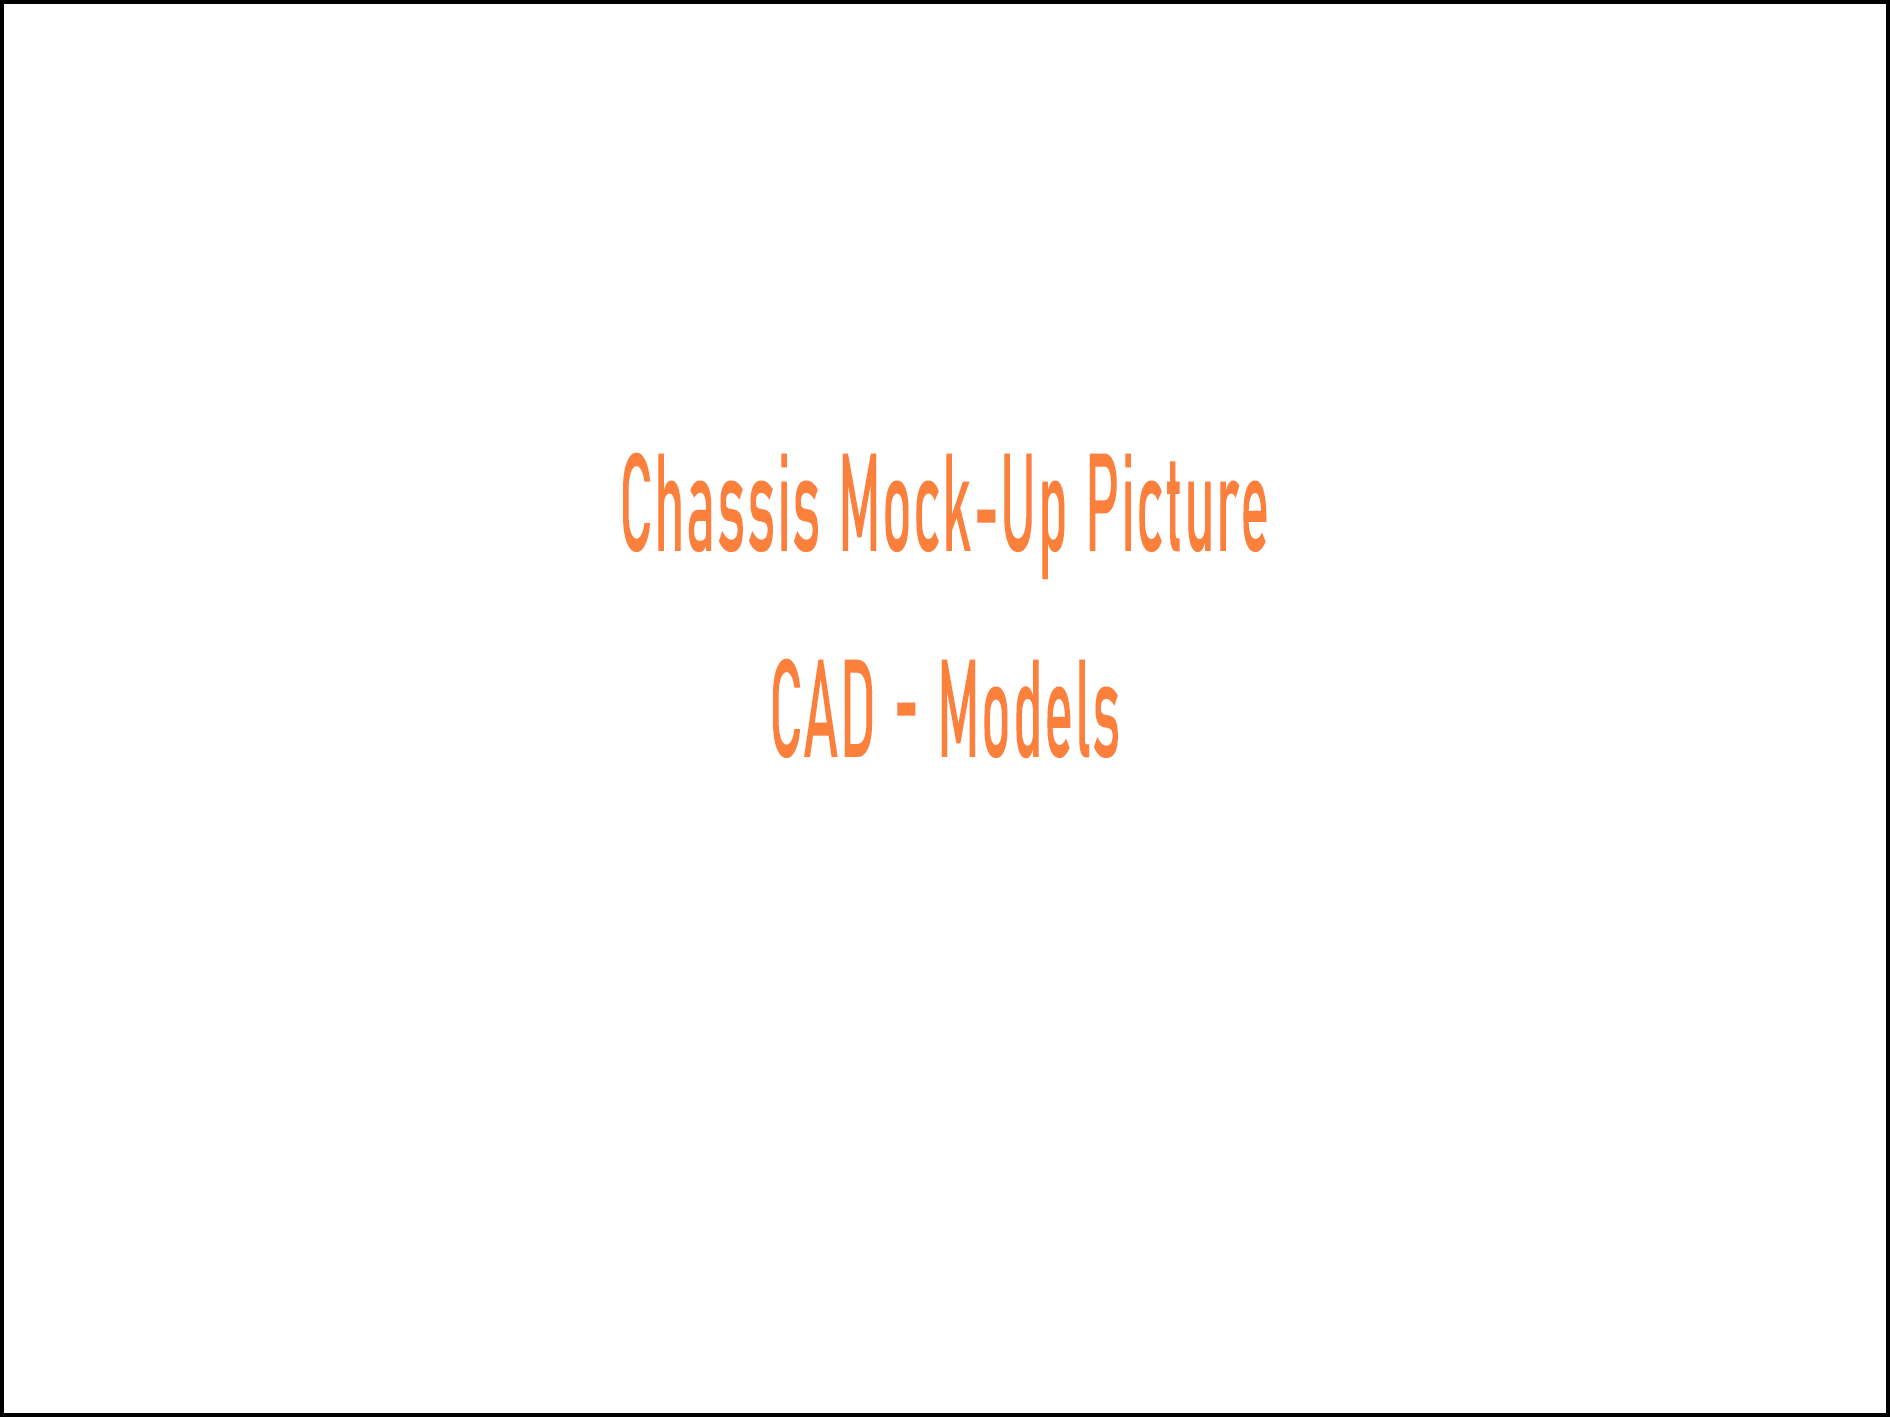
\includegraphics[width=\linewidth]{texfiles/mech/updated/chassis/cad1.png}
  \caption{Caption for the image.}
  \label{fig:image1}
\end{figure}

\begin{figure}[ht]
  \centering
  \begin{subfigure}{0.5\textwidth}
    \centering
    \includegraphics[width=\linewidth]{texfiles/mech/updated/chassis/technicaldrawing1}
    \caption{Caption for the first image.}
    \label{fig:sub1}
  \end{subfigure}%
  
  \begin{subfigure}{0.5\textwidth}
    \centering
    \includegraphics[width=\linewidth]{texfiles/mech/updated/chassis/technicaldrawing1}
    \caption{Caption for the second image.}
    \label{fig:sub2}
  \end{subfigure}
  \caption{Caption for the whole figure.}
  \label{fig:test}
\end{figure}

\begin{figure}[ht!]
  \centering
  \begin{subfigure}{.5\textwidth}
    \centering
    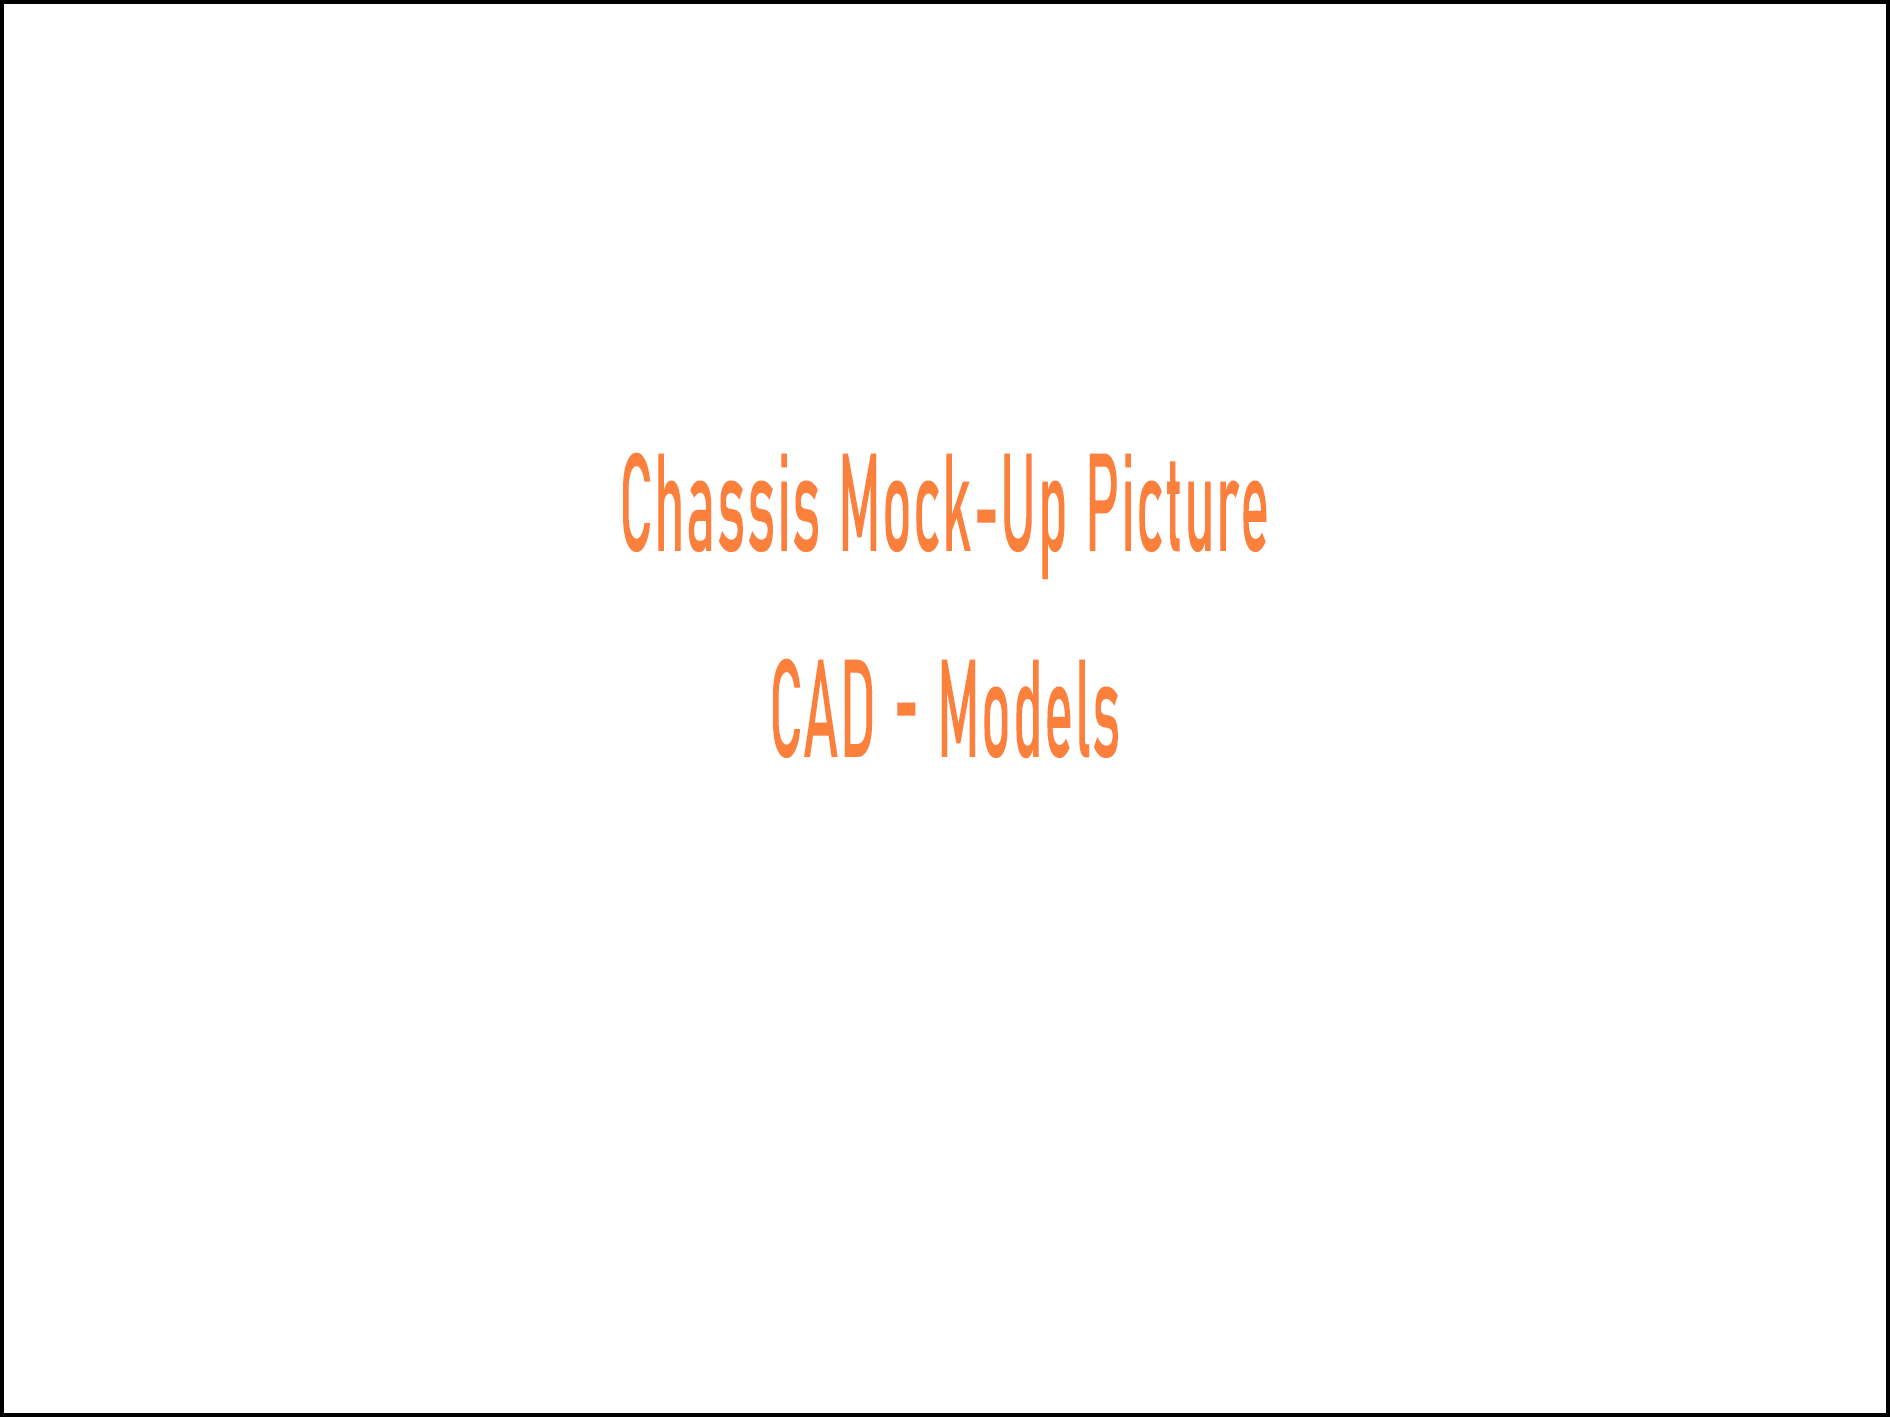
\includegraphics[width=\linewidth]{texfiles/mech/updated/chassis/cad1.png}
    \caption{Caption for the first image.}
    \label{fig:sub1}
  \end{subfigure}%
  \begin{subfigure}{.5\textwidth}
    \centering
    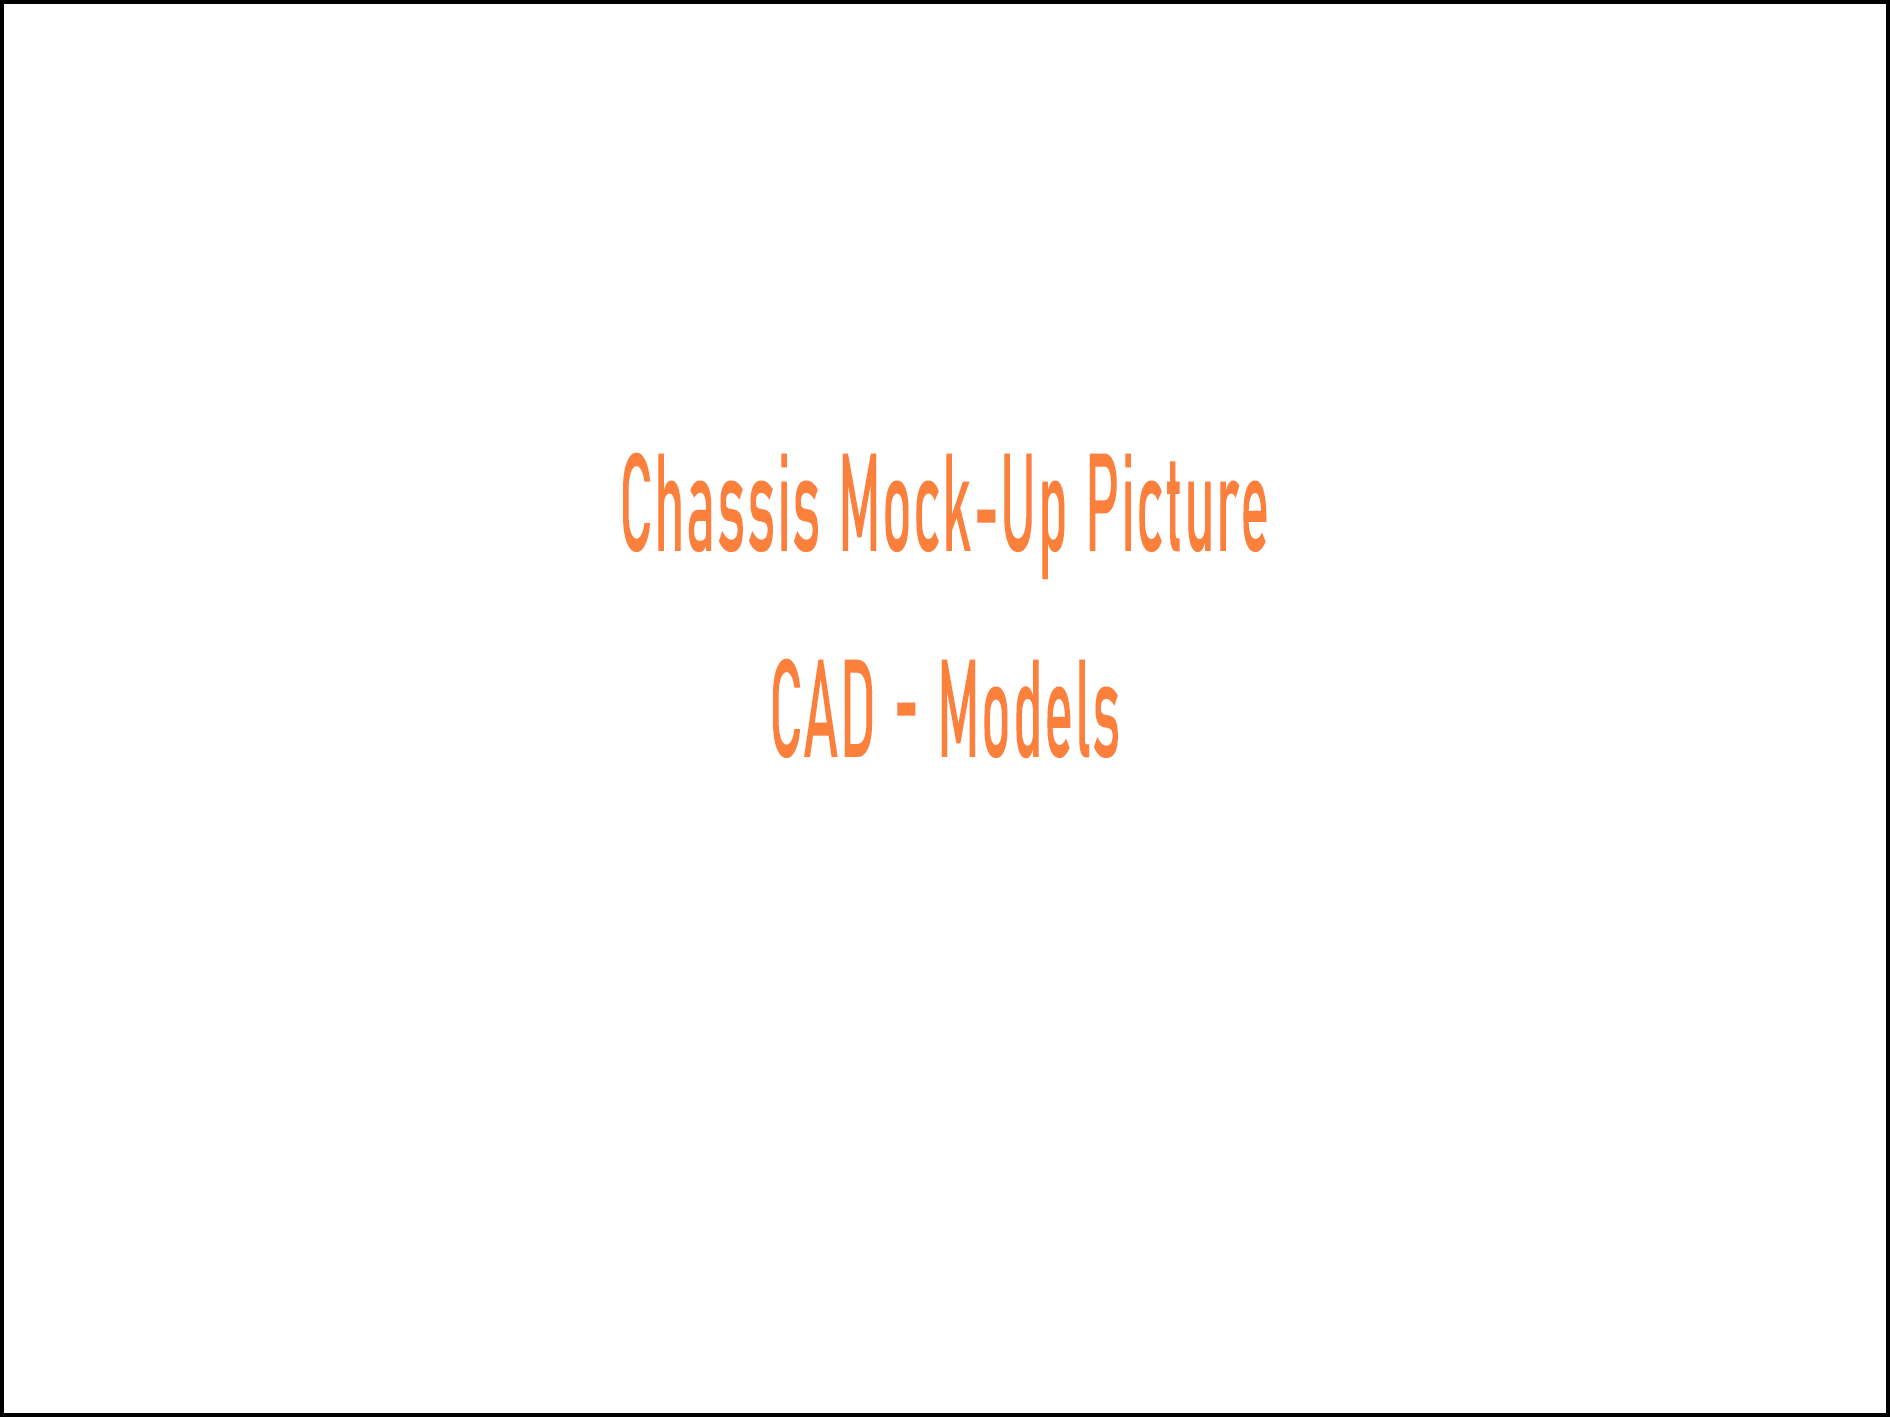
\includegraphics[width=\linewidth]{texfiles/mech/updated/chassis/cad1.png}
    \caption{Caption for the second image.}
    \label{fig:sub2}
  \end{subfigure}
  \caption{Caption for the whole figure.}
  \label{fig:test}
\end{figure}

\end{comment}
\subsubsection{Materials}
\textbf{WILL BE ADDED SOON}
\subsubsection{Design Rationale}


The design rationale guiding our pod's infrastructure embodies a methodical process rooted in practical considerations and engineering principles. Our primary aim was to reduce weight from the previous design, leading us to explore the potential of carbon fiber composites.
Initially, a monocoque chassis was considered for its structural integrity, yet its high cost and manufacturing complexity deemed it impractical. Similarly, the idea of a tube chassis with carbon fiber tubes proved prohibitively expensive.
Thus, we opted for a Composite Sandwich Panel Chassis, renowned for its lightweight, structural strength, and cost-effectiveness. Departing from the original design, which featured longitudinal panels spanning the entire length of the pod, we recognized the necessity for easy battery extraction from the side, prompting a redesign of the chassis layout.
To ensure seamless panel interlocking and structural integrity, we devised a plug-in system featuring evenly distributed cutouts, meticulously aligned for connection. These connections are strengthened by precise gluing and reinforced seaming along the edges.
Additionally, crossbars were strategically integrated to fortify the chassis at suspension mounting points, mitigating potential structural weaknesses.
Furthermore, close collaboration between the chassis department and other subsystems facilitated maximal compatibility and integration.
In summary, our design rationale represents a pragmatic synthesis of innovation and engineering expertise, driven by a commitment to efficiency, functionality, and cost-effectiveness.

\subsubsection{FEM Results}
\textbf{WILL BE ADDED SOON}
\begin{comment}
\begin{figure}[ht]
  \centering
  \includegraphics[width=\linewidth]{texfiles/mech/updated/chassis/fem1.png}
  \caption{Caption for the image.}
  \label{fig:image1}
\end{figure}

\begin{figure}[ht]
  \centering
  \begin{subfigure}{.5\textwidth}
    \centering
    \includegraphics[width=\linewidth]{texfiles/mech/updated/chassis/fem1.png}
    \caption{Caption for the first image.}
    \label{fig:sub1}
  \end{subfigure}%
  \begin{subfigure}{.5\textwidth}
    \centering
    \includegraphics[width=\linewidth]{texfiles/mech/updated/chassis/fem1.png}
    \caption{Caption for the second image.}
    \label{fig:sub2}
  \end{subfigure}
  \caption{Caption for the whole figure.}
  \label{fig:test}
\end{figure}
\end{comment}
\subsubsection{Calculations}
\textbf{WILL BE ADDED SOON}
\subsubsection{Mesh and Boundary Conditions}
\textbf{WILL BE ADDED SOON}
\begin{comment}
\begin{figure}[ht]
  \centering
  \begin{subfigure}{.5\textwidth}
    \centering
    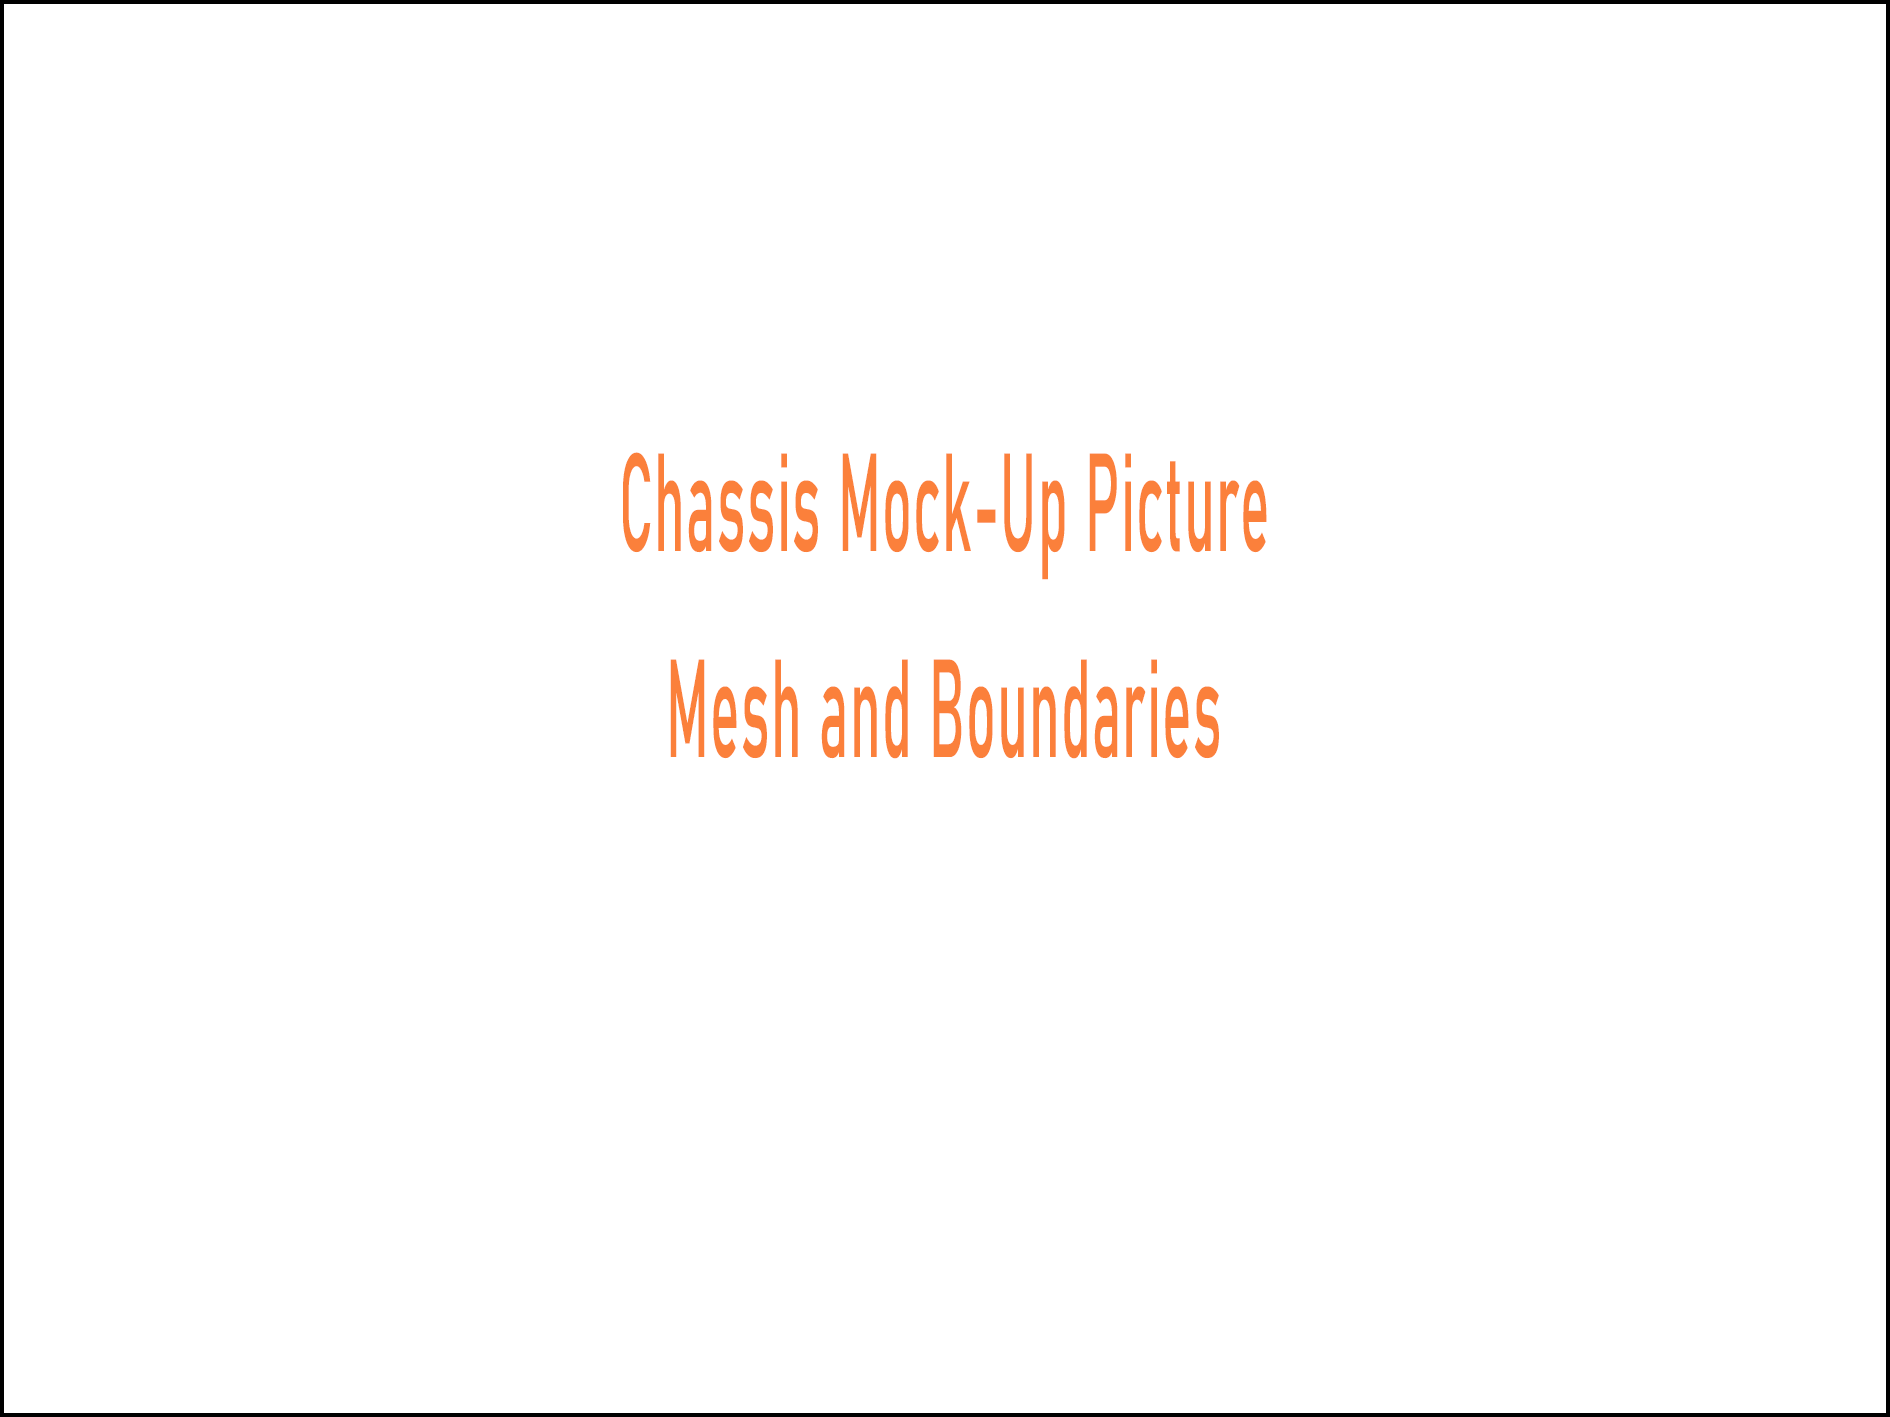
\includegraphics[width=\linewidth]{texfiles/mech/updated/chassis/Mesh1.png}
    \caption{Caption for the first image.}
    \label{fig:sub1}
  \end{subfigure}%
  \begin{subfigure}{.5\textwidth}
    \centering
    \includegraphics[width=\linewidth]{texfiles/mech/updated/chassis/mesh1.png}
    \caption{Caption for the second image.}
    \label{fig:sub2}
  \end{subfigure}
  \caption{Caption for the whole figure.}
  \label{fig:test}
\end{figure}
\end{comment}

\subsection{Manufacturing Process}


Firstly, the panels are sourced and procured in accordance with precise specifications, ensuring they meet the required size and shape criteria. Any necessary cutouts or holes are meticulously made in alignment with design specifications, utilizing advanced cutting techniques to ensure accuracy and consistency.
Subsequently, support plates are precisely cut to the required size and shape, with corresponding holes carefully drilled to facilitate seamless integration with the panels. These support plates serve a critical role in reinforcing the structural integrity of the chassis, providing additional strength and stability.
Following preparation of the panels and support plates, a meticulous assembly process ensues. The support plates are methodically glued to the designated spots on the panels, adhering to precise positioning guidelines to ensure optimal alignment and functionality.
Once the support plates are securely affixed, the panels are carefully assembled and glued together, forming a cohesive structure that embodies the desired design configuration. This assembly process is executed with meticulous attention to detail, ensuring that each component is seamlessly integrated to achieve the desired structural integrity and functionality.
Finally, the seams between the assembled panels are meticulously cut to the required size and adhered to the edges of the plugged panels. This final step serves to further reinforce the structural integrity of the chassis while providing a polished finish that enhances both aesthetics and durability.
Through adherence to this comprehensive manufacturing process, we ensure that the designed part is not only realized in a practical and efficient manner but also upholds the highest standards of quality and performance.



\subsection{Integration process}
\subsubsection{Assembling}


Firstly, the panels are sourced and procured in accordance with precise specifications, ensuring they meet the required size and shape criteria. Any necessary cutouts or holes are meticulously made in alignment with design specifications, utilizing advanced cutting techniques to ensure accuracy and consistency.

Subsequently, support plates are precisely cut to the required size and shape, with corresponding holes carefully drilled to facilitate seamless integration with the panels. These support plates serve a critical role in reinforcing the structural integrity of the chassis, providing additional strength and stability.

Following preparation of the panels and support plates, a meticulous assembly process ensues. The support plates are methodically glued to the designated spots on the panels, adhering to precise positioning guidelines to ensure optimal alignment and functionality.

Once the support plates are securely affixed, the panels are carefully assembled and glued together, forming a cohesive structure that embodies the desired design configuration. This assembly process is executed with meticulous attention to detail, ensuring that each component is seamlessly integrated to achieve the desired structural integrity and functionality.

Finally, the seams between the assembled panels are meticulously cut to the required size and adhered to the edges of the plugged panels. This final step serves to further reinforce the structural integrity of the chassis while providing a polished finish that enhances both aesthetics and durability.

Through adherence to this comprehensive manufacturing process, we ensure that the designed part is not only realized in a practical and efficient manner but also upholds the highest standards of quality and performance.

\subsubsection{Assembly interaction}


The interaction between subsystems within the pod is orchestrated with precision, each component playing a crucial role in ensuring seamless functionality and performance.
At the heart of this interaction lies the chassis, serving as the sturdy backbone upon which all subsystems are mounted. The chassis not only provides structural support but also serves as a conduit for distributing forces generated by key subsystems such as the brakes, motor, and suspension.
The motor, positioned centrally within the pod, exerts significant forces that are channeled directly through the chassis. As the primary source of propulsion, the motor's torque and power output directly influence the chassis's stability and performance.
Similarly, the braking system, situated on the sides directly above the track, exerts substantial forces during deceleration. These forces are transmitted through the chassis, requiring robust structural reinforcement to withstand the resulting stresses.
The suspension system, located at the front and back ends of the pod, plays a critical role in ensuring ride comfort and handling. The forces generated by the suspension, particularly during cornering and uneven terrain traversal, are transmitted through the chassis, necessitating careful design considerations to maintain stability and responsiveness.
In addition to these dynamic subsystems, the electrical systems are integrated into the chassis using sheet metal and 3D-printed brackets. This strategic mounting ensures secure placement while minimizing interference with other components.
Furthermore, the battery, housed within a dedicated battery box, is mounted on telescopic rails affixed to the chassis. This arrangement not only facilitates easy access for maintenance but also ensures optimal weight distribution and stability.
Through integration and strategic mounting, each subsystem interacts harmoniously with the chassis and other components, collectively contributing to the overall functionality and performance of our pod. This cohesive interaction is essential for achieving our objectives of efficiency, reliability, and safety.



\subsection{Safety Considerations}
\subsubsection{Safety Factor}
\textbf{WILL BE ADDED SOON}
\subsubsection{Worst-Case Scenarios}
\textbf{WILL BE ADDED SOON}
\subsection{FMEA Results Discussion}
\subsubsection{Risk Assessment}
\textbf{WILL BE ADDED SOON}
\subsubsection{FMEA and Risk Mitigation}
\textbf{WILL BE ADDED SOON}

\begin{figure}[ht]
  \centering
  \includegraphics[width=\linewidth]{texfiles/mech/updated/chassis/fmea1.png}
  \caption{Caption for the image.}
  \label{fig:image1}
\end{figure}

\subsubsection{Simulation Evidence}
\textbf{WILL BE ADDED SOON}


\subsection{Testing}
\subsubsection{Safety Procedures Documentation}


The testing procedures for the hyperloop pod chassis are meticulously crafted to assess structural integrity, durability, and performance under conditions that closely simulate actual operation. The procedures outlined below provide a comprehensive approach to validating the chassis design.

\paragraph{Static Load Testing}
\begin{itemize}
    \item \textbf{Objective:} To evaluate the chassis's ability to withstand forces it would encounter while stationary.
    \item \textbf{Procedure:} Securely mount the chassis at suspension mounting holes. Apply a static load equivalent to twice the anticipated weight of the finished pod.
    \item \textbf{Outcome:} Determine load-bearing capacity and ensure no structural deformation or failure.
\end{itemize}

\paragraph{Dynamic Load Testing}
\begin{itemize}
    \item \textbf{Objective:} To assess the chassis's responsiveness and robustness under dynamic loading conditions.
    \item \textbf{Procedure:} Subject the chassis to simulated forces of acceleration, braking, and cornering. Collect data on how the chassis flexes and reacts under these conditions.
    \item \textbf{Outcome:} Confirm the chassis's integrity under dynamic stresses and identify potential areas for reinforcement.
\end{itemize}

\paragraph{Bending Stress Test}
\begin{itemize}
    \item \textbf{Objective:} To understand the material properties of the chassis, particularly its bending strength and ductility.
    \item \textbf{Procedure:} Fabricate a reference part from the same material as the chassis. Apply incremental force until the part fails, if applicable.
    \item \textbf{Outcome:} Ascertain the material's resistance to bending forces and its behavior under stress.
\end{itemize}

\paragraph{Vibration Testing}
\begin{itemize}
    \item \textbf{Objective:} To evaluate the chassis's ability to endure and dampen vibrations during operation.
    \item \textbf{Procedure:} Expose the chassis to controlled vibrations at various frequencies and amplitudes to simulate motor-generated vibrations and other operational scenarios.
    \item \textbf{Outcome:} Ensure the chassis can effectively dampen vibrations and avoid resonance or structural fatigue.
\end{itemize}

\subsubsection{preliminary testing plan}

This section outlines the testing plan for the chassis of the hyperloop pod, ensuring its structural integrity and stability under various loads and conditions.

\paragraph{Static Load Testing}
\begin{itemize}
    \item \textbf{Method:} Securely mount the chassis at the suspension mounting holes.
    \item \textbf{Loading:} Apply a static load equivalent to twice the weight of the finished pod.
    \item \textbf{Duration:} Maintain the load for a predetermined period to assess the structural integrity.
    \item \textbf{Measurement:} Monitor for deformation or failure.
\end{itemize}

\paragraph{Dynamic Load Testing}
\begin{itemize}
    \item \textbf{Method:} Simulate dynamic forces experienced during operation.
    \item \textbf{Loading:} Apply forces to replicate acceleration, braking, and cornering.
    \item \textbf{Duration:} Perform over various speeds and conditions.
    \item \textbf{Measurement:} Record deflection and structural response.
\end{itemize}

\paragraph{Bending Stress Test}
\begin{itemize}
    \item \textbf{Method:} Use a reference part made from the same material as the chassis panels.
    \item \textbf{Loading:} Incrementally apply force until failure.
    \item \textbf{Measurement:} Note the force applied and deformation at failure.
    \item \textbf{Expected Result:} Determine material's bending strength and ductility.
\end{itemize}

\paragraph{Vibration Testing}
\begin{itemize}
    \item \textbf{Method:} Subject chassis to controlled vibrations across frequencies.
    \item \textbf{Loading:} Simulate operational vibrations.
    \item \textbf{Duration:} Extend testing for durability assessment.
    \item \textbf{Measurement:} Assess chassis damping and response to vibrations.
    \item \textbf{Expected Result:} Ensure chassis can maintain integrity under vibration.
\end{itemize}

\paragraph{Expected Results}
The chassis is expected to demonstrate stability and maintain structural integrity under static and dynamic loads. The bending stress test will confirm the material's properties, while vibration testing will validate damping capabilities. Through this comprehensive testing, the chassis will be proven to meet rigorous quality and safety standards, crucial for the hyperloop pod's performance.
